\documentclass[conference]{IEEEtran}
\IEEEoverridecommandlockouts
\usepackage{fontspec}
\usepackage{amsmath}
\usepackage{unicode-math}
\setmainfont{STIX Two Text}
\setmathfont{STIX Two Math}
\usepackage{cite}
\usepackage{graphicx}
\usepackage{textcomp}
\usepackage{xcolor}
\usepackage{booktabs,array}
\usepackage{url}
\usepackage[shortlabels]{enumitem}
\setlist{nosep,leftmargin=*,topsep=1pt}
\newcommand{\Nsub}{8}

\begin{document}

\title{Category and Load Effects in HCP Working Memory and Language Task-fMRI: \\ A Pattern-Based Model of Task Demands}

\author{\IEEEauthorblockN{1\textsuperscript{st} Sai Veeksha Tavva}
\IEEEauthorblockA{\textit{IIIT Hyderabad} \\
Roll No.\ 2024113021}
\and
\IEEEauthorblockN{2\textsuperscript{nd} Sahishnu Pawan Kumar}
\IEEEauthorblockA{\textit{IIIT Hyderabad} \\
Roll No.\ 2024113016}
}

\maketitle

\begin{abstract}
Working-memory tasks make two kinds of demand on the brain: how much is held (\emph{load}) and what is held (\emph{category}, e.g.\ faces or places). We ask which regions carry each kind of information and whether the code for one survives a change in the other, using Human Connectome Project data from eight people and our own analysis code. Category could be read out reliably from early visual and visual-object cortex, and less securely from parietal cortex. In visual regions most of it was kept when load rose from 0-back to 2-back, but some was lost, and we could not show the code is unchanged. Load could be read out from seven of eight regions, and in prefrontal and parietal cortex as a spatial pattern, not only as overall activity. A decoder trained on hard versus easy memory blocks also told Math from Story in a separate language task in prefrontal, parietal, cingulate and auditory association cortex, suggesting a shared demand signal. Against resting-state scans from four of the eight people with the same task timing laid over them, the visual category result and load in five regions held; parietal category and load in early visual cortex did not, even with shifted timing and block position removed. With eight people, this is a pilot. Code: \url{https://github.com/veeksha12/incm-hcp-task-fmri-project}.
\end{abstract}

\begin{IEEEkeywords}
working memory, task fMRI, representational similarity analysis, decoding, representational geometry
\end{IEEEkeywords}

\section{Aim of the Modelling Exercise}
We build and test a quantitative, pattern-based model of how the brain's response to a working-memory (WM) task is organised by a domain-general demand (memory \emph{load}) and a content-specific demand (the \emph{category} held: faces, places, tools, body parts). Using Human Connectome Project (HCP) task-fMRI, we ask: do multivoxel patterns differ between categories, does this information persist when load rises from 0-back to 2-back, and is the load signal shared between a visual task (N-back) and an auditory one (Language: Math versus Story)? Each hypothesis has a pre-specified analysis and null:
\begin{itemize}
\item \textbf{H1 (category patterns).} Each category evokes a distinct, reproducible pattern in occipito-temporal (OT) cortex, distributed rather than carried only by the most selective voxels.
\item \textbf{H2 (dissociation, invariance).} Load is carried mainly by frontoparietal and cingulate regions, category by OT cortex, and the category code is preserved across load.
\item \textbf{H3 (control).} Both effects exceed a null built from resting-state fMRI (rfMRI) run through the same pipeline.
\item \textbf{H4 (modality-general demand).} A 2-back versus 0-back pattern learned in vision transfers to Math versus Story in frontoparietal but not sensory cortex.
\end{itemize}
\textbf{Scope.} \Nsub{} HCP participants, two runs each (LR, RL), eight bilateral Glasser-parcellation ROIs. Inference treats the participant as the unit.

\section{Introduction and Motivation}
The HCP WM task is an N-back task with faces, places, tools and body parts in separate blocks, half at 0-back and half at 2-back \cite{vanessen2013,barch2013}; its activations are reliable \cite{drobyshevsky2006,barch2013}. Averaged over category, 2-back versus 0-back engages a frontoparietal ``multiple-demand'' system \cite{duncan2010}; averaged over load, category contrasts recover face-, place- and body-selective OT regions \cite{kanwisher1997,epstein1998,downing2001}. Three questions remain. \emph{(i) Where and how is category coded?} Haxby \emph{et al.}\ \cite{haxby2001} found a distributed code in six subjects and a one-back task; whether HCP WM data agree needs pattern analysis such as RSA \cite{kriegeskorte2008}. \emph{(ii) What does load do to the category code?} It could sharpen, compress or distort the representational geometry, or change only its scale \cite{emrich2013,kriegeskorte2013,bernardi2020}; average activation cannot tell these apart. \emph{(iii) Is demand specific to vision?} If frontoparietal cortex carries a modality-general signal, a load pattern should also separate Math from Story \cite{binder2011}. We claim no novelty for individual methods; the contribution is their combination, with controls (Section~\ref{sec:novelty}).

\textbf{Model.} Stage 1 (encoding): at each grayordinate the series is a linear response to the block design,
\begin{equation}
y(t)=\sum_{k}\beta_k\,(s_k\ast h)(t)+\text{drift}(t)+\text{motion}(t)+\varepsilon(t),
\label{eq:glm}
\end{equation}
with $\varepsilon_t=\rho\,\varepsilon_{t-1}+u_t$, condition indicators $s_k$ (eight WM conditions, two Language) and a double-gamma haemodynamic response $h$; the $\beta_k$ or $t$-values over an ROI form pattern $\mathbf{p}_k$. Stage 2 (representational): the pattern for category $c$ at load $l$ is a shared code scaled by a load gain, plus a load offset and noise,
\begin{equation}
\mathbf{p}_{c,l}=\mathbf{m}_l+g_l\,\mathbf{s}_c+\boldsymbol{\eta}_{c,l}.
\label{eq:rep}
\end{equation}
$g_2<g_0$ means load weakens the code, $g_2=g_0$ with the same $\mathbf{s}_c$ means invariance, and a change in $\mathbf{m}_l$ alone is a pure load effect. Table~\ref{tab:variations} lists our variations on the standard baseline (GLM, RDMs from beta maps, linear decoder; Neuromatch HCP exercise), which we reproduce.

\begin{table}[!tb]
\caption{Variations relative to the baseline pipeline.}
\label{tab:variations}
\centering\footnotesize
\renewcommand{\arraystretch}{1.05}
\begin{tabular}{@{}p{0.45cm}p{2.0cm}p{5.5cm}@{}}
\toprule
 & \textbf{Baseline} & \textbf{Our variation (motivation)}\\
\midrule
V1 & Library GLM. & Own design matrix, AR(1) prewhitening vs.\ OLS (serial correlation inflates $t$ \cite{woolrich2001}).\\
V2 & RDM from beta correlations. & Own NumPy cross-run cross-validated distances (expected value zero without signal \cite{walther2016,nili2014}).\\
V3 & One rank correlation over six pairs. & Full $8\times8$ RDM with transfer, gain and an equivalence (TOST) test (a non-significant difference is not invariance).\\
V4 & Chance as only reference. & Matched rfMRI null: same design and pipeline on resting data.\\
V5 & Within-task decoding. & Leave-one-subject-out, cross-load, cross-task decoding and a demand-axis correlation (tests H4 directly).\\
V6 & Face-value accuracy. & ROI mean removed \cite{coutanche2013}; timing audit; fold-local scaling; participant-level sign-flip and FDR \cite{stelzer2013,nichols2002}.\\
\bottomrule
\end{tabular}
\end{table}

\textbf{Difference from class models.} The class models (passive membrane, integrate-and-fire, Hodgkin--Huxley, FitzHugh--Nagumo) are \emph{mechanistic}: differential equations integrated in time and compared with voltage or spikes. Ours is \emph{descriptive and representational}: latent quantities are pattern vectors and gains, the observable is the haemodynamic signal at 91{,}282 grayordinates (TR $0.72$\,s), the dynamics are a linear HRF convolution with AR(1) noise followed by a static stage, and evaluation is by cross-validation, permutation, rfMRI nulls and equivalence tests. The mathematics is shared: the passive membrane is a first-order low-pass filter turning a current step into a delayed, smoothed voltage, as the HRF in \eqref{eq:glm} does for neural activity. We do not simulate spiking or synaptic dynamics; a model of activity-silent maintenance is future work. Our claims concern information in measured patterns, not cellular mechanism.

\section{Methods}
All analyses are in Python (NumPy, SciPy, scikit-learn) in one notebook; GLM, representational analysis and permutation tests are our own implementations. Seeds are fixed.

\textbf{Data.} \Nsub{} unrelated participants of the HCP 1200 release \cite{vanessen2013}, each with LR and RL runs of the WM (405 frames) and Language (316 frames) tasks \cite{barch2013,binder2011}; four also have resting-state runs. We used minimally pre-processed CIFTI data, MSMAll-aligned \cite{robinson2014} and ICA-FIX cleaned \cite{salimi2014}, with TR $=0.72$\,s (the CIFTI header value of 1.0\,s is wrong and overridden). Block timing comes from the HCP EV files and motion from \texttt{Movement\_Regressors}.

\textbf{Stage-1 GLM.} Per run and grayordinate we fit \eqref{eq:glm}: one regressor per condition, 12 motion terms, a 128\,s discrete-cosine high-pass basis and an intercept. We fit OLS, estimate the lag-1 residual autocorrelation $\rho$, bin it (0.005), whiten data and design per bin, and refit \cite{woolrich2001}. The runs are never merged in cross-run analyses.

\textbf{ROIs.} Eight bilateral Glasser ROIs \cite{glasser2016}, fixed before decoding: early visual (EVC; 3{,}632 grayordinates), ventral and lateral OT (1{,}850; 788), early and association auditory (1{,}187; 2{,}274), dorsolateral frontoparietal (FP\textsubscript{dlpfc}; 3{,}318), parietal (FP\textsubscript{parietal}; 2{,}460) and cingulate/pre-SMA (1{,}547). Sizes differ about fourfold, so ROI comparisons are descriptive.

\textbf{Split-half RSA.} For each participant and ROI the LR and RL $t$-maps of the eight conditions give $A,B\in\mathbb{R}^{8\times V}$. \emph{Identification:} after centring across categories within load, a condition is identified when its own cross-run pattern correlates highest (pairwise, chance $0.5$; cross-load uses 0-back from one run and 2-back from the other). \emph{Cross-validated distance:} $d_{ij}=\tfrac1V(\mathbf a_i-\mathbf a_j)^{\!\top}(\mathbf b_i-\mathbf b_j)$, symmetrised over runs \cite{walther2016,nili2014}; $\mathbb E[d_{ij}]=0$ without a reproducible difference. No spatial whitening was applied (a limitation); unit tests cover symmetry, zero diagonal and signal/noise behaviour. \emph{Distributed code:} grayordinates ranked by an $F$ statistic in one run were removed in the other (0--70\,\%) and compared with 100 random removals \cite{haxby2001}. For Language (two conditions) we report only the cross-run reliability of Math$-$Story.

\textbf{LOSO decoding.} A dual-form ridge classifier ($\lambda=\mathrm{tr}(K)/n$, one-versus-rest) is trained on all other participants and tested on the held-out one, on single-block $t$-maps with fold-local scaling; targets are category (chance 0.25), load (0.5) and Math/Story (0.5). A linear SVM cross-checks the ridge form. \emph{Cross-load:} train on one load, test on the other, and repeat with each category left out in turn. \emph{Permutation null:} 1000 within-structure label permutations rerunning the full LOSO; bootstrap intervals resample participants, never blocks.

\textbf{Pattern versus amplitude.} Decoders can exploit ROI-mean differences \cite{coutanche2013}; load and cross-task decoding were repeated after removing each block's ROI mean (300 permutations for load) and from the ROI mean alone. Information is called \emph{pattern} if it survives mean removal.

\textbf{Load invariance (H1/H2).} On the $8\times8$ cross-run RDM we compute, per participant and ROI, \emph{within-load distinctness} $\bar d_l$ (mean of the six category distances at load $l$); \emph{transfer} (mean cross-load different-category distance minus same-category distance, divided by the group-mean $(\bar d_0+\bar d_2)/2$; 1 is the same code, 0 none); and \emph{gain} $\bar d_2/\bar d_0$ (since $d\propto g_l^2$). Ratios are interpreted only where within-load distinctness is reliably above zero. The null permutes the $4!$ category correspondences between loads (5000 draws). For invariance we use two one-sided tests (TOST) \cite{schuirmann1987} with margins fixed beforehand ($\pm0.25$ for transfer, $\pm0.10$ for accuracy loss) and report the smallest margin at which equivalence would hold.

\textbf{Matched rfMRI null.} For the four participants with resting data we impose the real WM design on random 405-frame resting windows and rerun the pipeline (1000 draws for RSA statistics, with a group null from averaging one draw per person; 100 draws for decoding, so the smallest $p$ is $0.01$ and smallest FDR $q$ is $0.028$).

\textbf{Cross-task decoding and demand axis.} A ridge classifier trained on WM load in other participants is applied to the held-out participant's Language blocks (direction A), and vice versa (B), with Math $\leftrightarrow$ 2-back fixed beforehand; full, mean-removed and mean-only versions are judged separately. Inference is by exact sign-flip across participants ($2^n$ flips; smallest two-sided $p=0.0078$ at $n=8$) with Benjamini--Hochberg FDR \cite{benjamini1995}, and we report how many people exceed 0.5. The demand axis is the correlation, across grayordinates and between different runs, of the load pattern (2-back minus 0-back) with Math$-$Story, with an attenuation correction only where both reliabilities exceed 0.2. Category RDMs at the two loads are also compared by a Mantel test \cite{mantel1967} and a noise ceiling.

\textbf{Event-timing audit and controls.} Shared schedules can inflate cross-participant decoding. We compared block onsets across participants (``shared'' within 0.5\,s). The WM schedule is shared within about 0.32\,s; the Language schedule differs between people. For parietal category we also (a) shifted the task design circularly in time over random resting windows (1000 draws) and (b) regressed out each block's position in the run (linear, or linear plus quadratic) in task and resting data. These speak for the four people with resting data only.

\textbf{Approaches abandoned.} (1) A Spearman correlation over the six pairs of the two category RDMs was uninformative: the null spread was very wide (SD $\approx0.46$; $q\approx0.996$) and it cannot express equivalence; we replaced it with transfer, gain and TOST. (2) A block-level label-flip null for cross-task decoding was anti-conservative because blocks are not independent (the Math/Story pattern is almost the same across people); we replaced it with the participant-level sign-flip test. A verdict rule that declared ``no transfer'' when full-pattern accuracy was below 0.6 despite pattern-only transfer was also fixed.

\textbf{Limitations of the methods.} Not done: a spin permutation test (needs sphere files), resting controls for the other four people, more than 100 decoding draws outside parietal cortex, and the parietal ``unchanged across load'' test with places removed. No power calculation was done; ROI definitions are group-based.

\section{Results}
All results use \Nsub{} participants. Chance is $0.25$ for category (four classes) and $0.50$ for load and Math/Story; ``reliable'' (bold) means passing a test corrected for multiple comparisons.

\textbf{Preliminary checks.} In one person, regions more active at 2-back overlapped regions more active for Math than Story about 7.5 times more than chance (descriptive, no test). All eight saw WM blocks within about 0.3\,s of each other, and Language timing differed. Places blocks came late in both runs (correlation with time $+0.61$, $+0.51$), so places is the category most at risk of being confused with time.

\begin{table}[!tb]
\caption{Category and load decoding (other people's data). Cat.\ same/other: trained and tested at the same/other load; loss shown where category is readable. Load: easy versus hard, full pattern and with average activity removed. Bold: reliable.}
\label{tab:cat}
\centering\footnotesize
\setlength{\tabcolsep}{3.5pt}
\begin{tabular}{@{}lccccc@{}}
\toprule
 & \multicolumn{3}{c}{Category (0.25)} & \multicolumn{2}{c}{Load (0.50)}\\
\cmidrule(lr){2-4}\cmidrule(l){5-6}
Region & Same & Other & Loss & Full & Mean rem.\\
\midrule
EVC & \textbf{0.77} & \textbf{0.61} & 0.16 & \textbf{0.68} & \textbf{0.66}\\
OT ventral & \textbf{0.72} & \textbf{0.63} & 0.09 & \textbf{0.66} & 0.52\\
OT lateral & \textbf{0.63} & \textbf{0.52} & 0.11 & \textbf{0.64} & \textbf{0.61}\\
AUD early & 0.27 & 0.21 & -- & 0.61 & 0.58\\
AUD assoc & 0.31 & 0.25 & -- & \textbf{0.70} & \textbf{0.70}\\
FP dlpfc & 0.34 & 0.20 & -- & \textbf{0.71} & \textbf{0.72}\\
FP parietal & \textbf{0.50} & \textbf{0.47} & 0.03 & \textbf{0.77} & \textbf{0.79}\\
Cing/pre-SMA & 0.34 & 0.21 & -- & \textbf{0.66} & \textbf{0.64}\\
\bottomrule
\end{tabular}
\end{table}

\textbf{Category (H1).} Category was reliably readable in EVC, both OT regions and parietal cortex, and in no other region (Table~\ref{tab:cat}; Fig.~\ref{fig:decoding}). At 0-back accuracy was $0.81$ (EVC), $0.78$ (OT ventral), $0.69$ (OT lateral); parietal was weaker (${\sim}0.50$). Within a person, one run identified the other run's pattern $0.82$--$0.87$ of the time in the three visual regions (chance $0.50$), and no other region was reliable. The signal is distributed: with the half most category-selective locations removed, visual regions still identified category ${\sim}0.7$ of the time, though removal cost more than random removal, so the signal is spread but not evenly.

\textbf{Caution on parietal cortex.} When places were removed, parietal cross-load accuracy fell from $0.22$ to $0.05$ above chance (4 of 8 people above chance), while visual regions were unaffected. Together with the places--time correlation and the fact that the only parietal pairs that worked across load included places, part of the parietal category signal may come from task timing, not the pictures.

\begin{figure}[!tb]
\centering
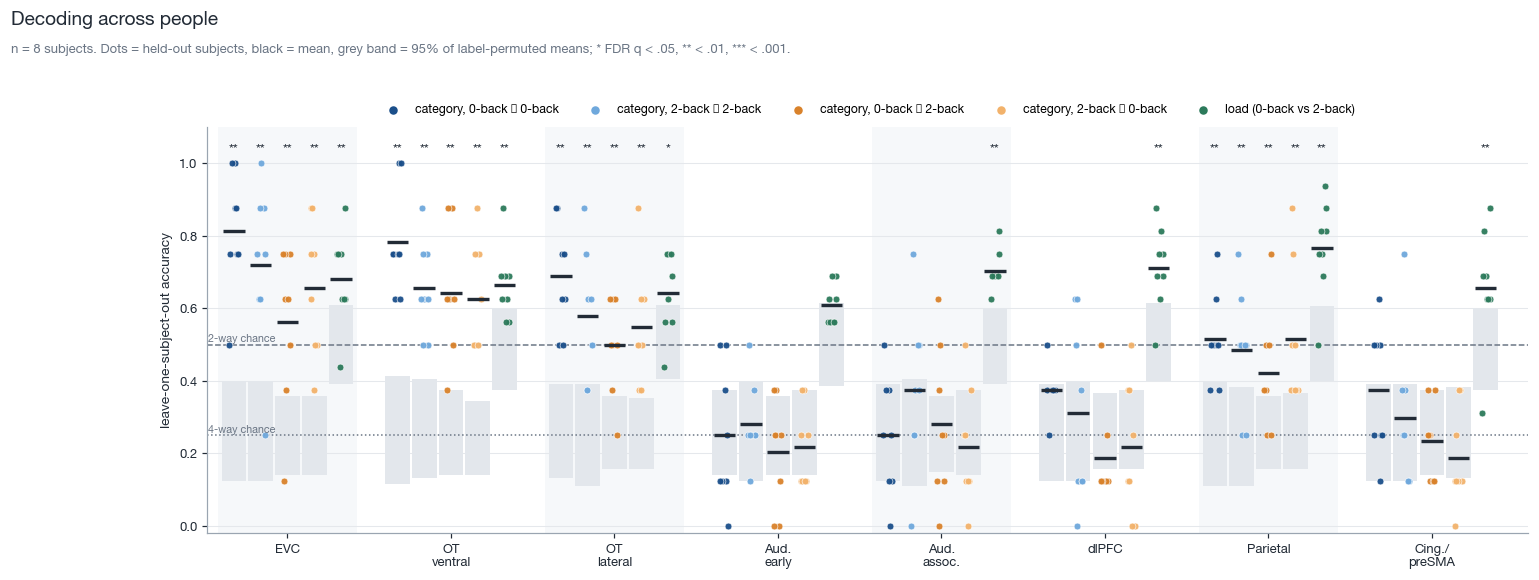
\includegraphics[width=\columnwidth]{figures/fig_decoding.png}
\caption{Category (same load, other load) and load decoding per region from other people's data. Each dot is one held-out person, the bar the average, grey bands what guessing gives, stars reliable results.}
\label{fig:decoding}
\end{figure}

\begin{figure}[!tb]
\centering
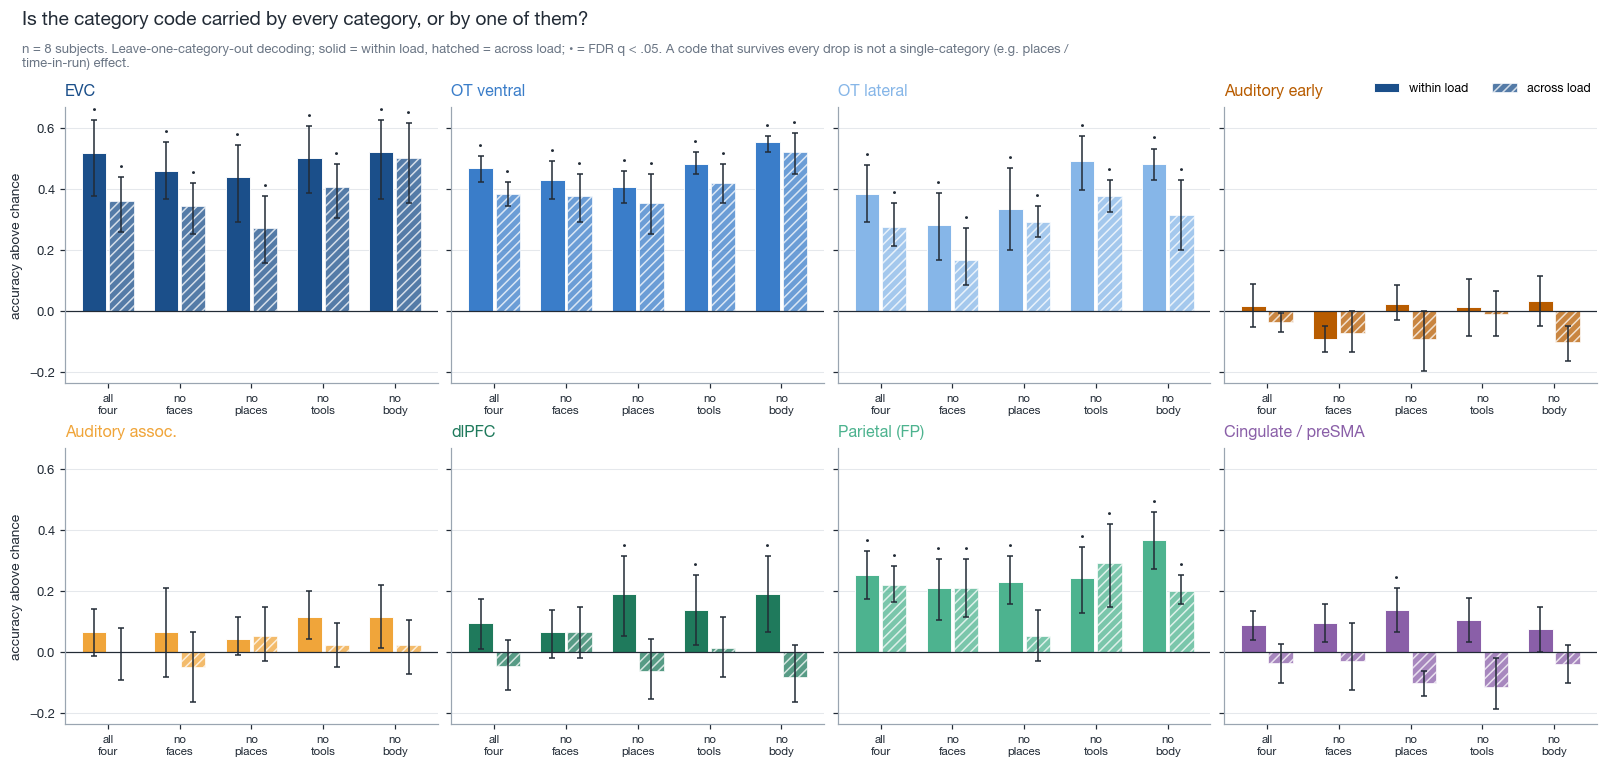
\includegraphics[width=\columnwidth]{figures/fig_leave_one_category.png}
\caption{Does the category code depend on one category? Bars: score above guessing with one category left out (solid: same load, hatched: other load); dots: reliable. Visual regions stay high; in parietal cortex the across-load score collapses when places is removed.}
\label{fig:loco}
\end{figure}

\textbf{Load (H2a).} Load was reliably readable in seven of eight regions ($0.64$--$0.77$; Table~\ref{tab:cat}), highest in parietal ($0.77$), prefrontal ($0.71$) and auditory association ($0.70$), though intervals overlap. In prefrontal and parietal cortex activity was higher at 2-back in nearly everyone (8/8, 7/8) and load survived removal of average activity, so the signal is a spatial pattern; the same held in auditory association cortex. In OT ventral, activity was lower at 2-back in all eight, and load vanished with the average removed: an overall activity change.

\textbf{Does the category code survive load (H2b)?} Visual regions kept most but not all category signal: loss was $0.16$ (EVC), $0.09$ (OT ventral), $0.11$ (OT lateral). Parietal lost only $0.03$, inside the $0.10$ margin set beforehand, but this did not survive correction over eight regions and leans on places. We cannot say the code is unchanged, nor that it changes: with eight people, showing sameness is much harder than showing a difference. The full-RDM analysis suggested one shared code of roughly constant strength in the visual regions; a rank comparison of category layout was suggestive in OT ventral, OT lateral and parietal but did not survive correction, and the SVM gave similar answers.

\begin{figure}[!tb]
\centering
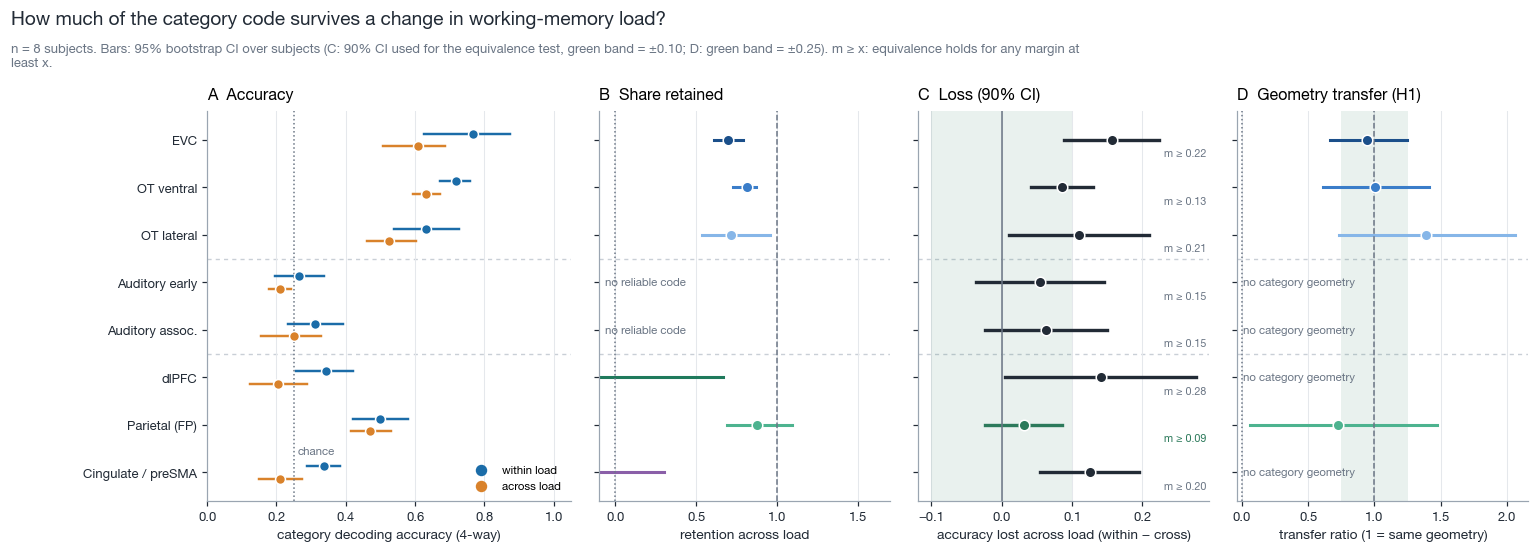
\includegraphics[width=\columnwidth]{figures/fig_load_survival.png}
\caption{How much of the category code survives a change in load? A: accuracy at the same and the other load. B: share of above-guessing accuracy that carries over. C: accuracy lost; green band is the margin set beforehand. D: similarity of category layout at the two loads.}
\label{fig:survival}
\end{figure}

\textbf{Resting-state check (H3).} For category across load, early visual and OT ventral beat the resting level ($p=0.001$, $q=0.004$) and OT lateral was borderline ($p=0.019$, $q=0.051$); parietal ($p=0.39$) and all other regions did not (Fig.~\ref{fig:rest-decoding}, Fig.~S1). Category decoding in EVC and OT ventral beat it in all four train/test combinations ($q=0.028$); parietal passed one (2-back to 2-back, $q=0.05$) and neither across-load one ($q\approx0.44$). Load beat the resting level in OT ventral, auditory association, prefrontal, parietal and cingulate ($q=0.028$) and just reached it in OT lateral ($q=0.05$), but not in EVC ($q=0.40$) or early auditory ($q=0.31$); parietal task accuracy was $0.89$ on these four people against about $0.50$ for rest. With four people and 100 draws, a failure to pass may partly reflect sample size. The older rank statistic could not separate signal from null anywhere.

\textbf{Parietal category against a schedule-only null.} Across load, accuracy never beat the schedule-shifted null in any version: $0.31$ both directions as analysed ($p=0.27$), after linear ($p=0.30$, $0.43$) and linear-plus-quadratic ($p=0.17$, $0.10$) position removal (Fig.~S7, Table~S1). Within a load results were unstable: 2-back to 2-back scored $0.50$ ($p=0.014$, $q=0.034$) but weakened under linear ($p=0.042$, $q=0.095$) and vanished under quadratic removal ($p=0.42$); 0-back to 0-back failed as analysed ($p=0.21$) and passed only after quadratic removal ($0.66$, $p=0.001$). A result that appears and disappears across versions, from four people and 32 test blocks, cannot be counted on; the across-load result that an ``unchanged code'' claim needs fails every time.

\begin{figure}[!tb]
\centering
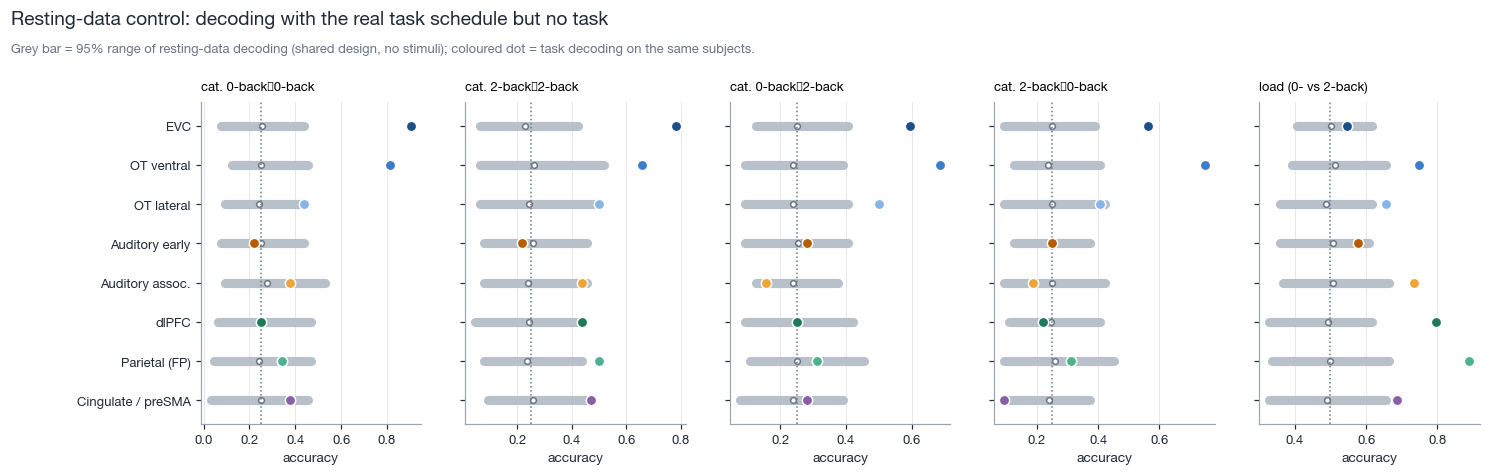
\includegraphics[width=\columnwidth]{figures/fig_rest_decoding.png}
\caption{Resting-data control for the decoders. Grey bar: range of scores with the real task timing laid over resting scans; dot: real task score for the same four people. Early visual and OT ventral stand out for category, and most regions except early visual and early auditory for load.}
\label{fig:rest-decoding}
\end{figure}

\begin{table}[!tb]
\caption{Load decoder applied to Language (Math treated as hard) with and without average activity, and correlation between the load and Math$-$Story patterns across separate runs. Bold: reliable.}
\label{tab:xt}
\centering\footnotesize
\setlength{\tabcolsep}{4pt}
\begin{tabular}{@{}lccc@{}}
\toprule
Region & Math/Story & Mean rem. & Pattern corr.\\
\midrule
EVC & 0.88 & 0.88 & 0.09\\
OT ventral & 0.75 & 0.63 & \textbf{0.07}\\
OT lateral & 0.81 & 0.81 & \textbf{0.18}\\
AUD early & 0.75 & 0.31 & 0.05\\
AUD assoc & \textbf{1.00} & \textbf{1.00} & \textbf{0.12}\\
FP dlpfc & \textbf{1.00} & \textbf{0.94} & \textbf{0.24}\\
FP parietal & \textbf{1.00} & \textbf{1.00} & \textbf{0.43}\\
Cing/pre-SMA & \textbf{0.94} & \textbf{0.94} & \textbf{0.21}\\
\bottomrule
\end{tabular}
\end{table}

\textbf{Shared demand signal (H4).} A load decoder trained on other people told Math from Story reliably in auditory association, prefrontal, parietal ($1.00$, all eight people) and cingulate ($0.94$) cortex, surviving removal of average activity (Table~\ref{tab:xt}); visual and early auditory regions were above $0.5$ but not reliable. Math was never labelled easy. Because Story versus Math is itself readable at about $1.00$ there, this shows agreement in direction more than an identical pattern. The reverse direction was weaker ($0.58$--$0.67$), reliable in OT ventral, OT lateral and prefrontal cortex, and in the two visual regions through average activity, not pattern. The demand-pattern correlation, free of the ceiling problem, was largest in parietal ($0.43$), then prefrontal ($0.24$) and cingulate ($0.21$), small but above zero in OT lateral, auditory association and OT ventral, and null in EVC and early auditory; the load pattern was not very repeatable between runs outside prefrontal and parietal cortex, weakening those correlations by an unknown amount.

\begin{figure}[!tb]
\centering
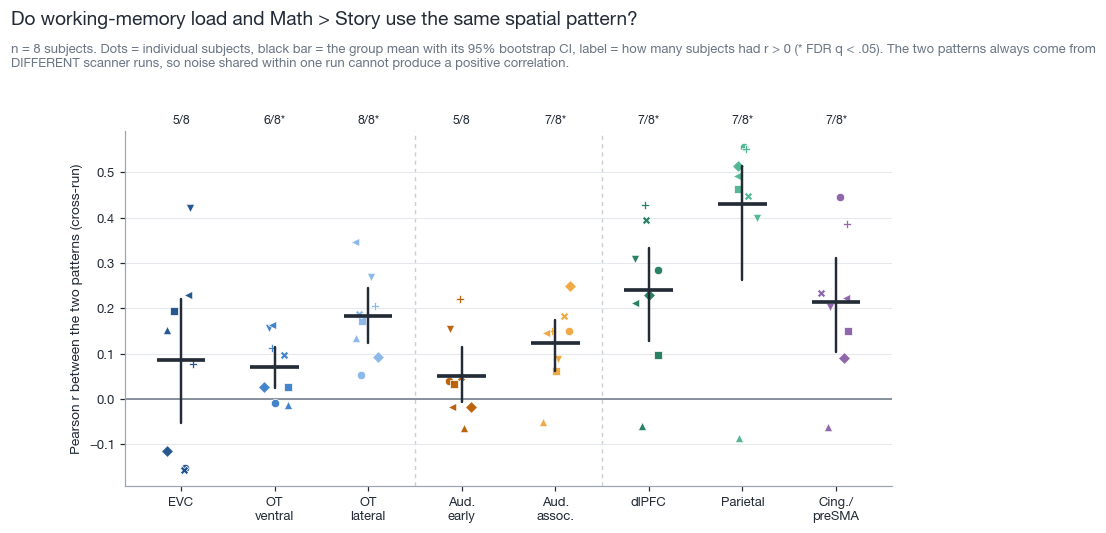
\includegraphics[width=\columnwidth]{figures/fig_demand_pattern.png}
\caption{Do memory load and Math versus Story share a spatial pattern? Each symbol is one person, the bar the group mean with its interval, the label the number of people with a positive correlation (star: reliable). Patterns come from different runs; parietal is largest.}
\label{fig:demand}
\end{figure}

\textbf{Summary.} H1 is supported in visual regions. H2a is partly supported (no clean split between regions). H2b is not established. H3 is partly supported: visual category and load in five regions beat the resting level, parietal category and early visual load do not. H4 is partly supported (reverse direction weak). Open: whether the code is unchanged across load, whether parietal category information is real, and resting controls for the other four people. Fig.~\ref{fig:summary} gathers the main numbers.

\begin{figure*}[!tb]
\centering
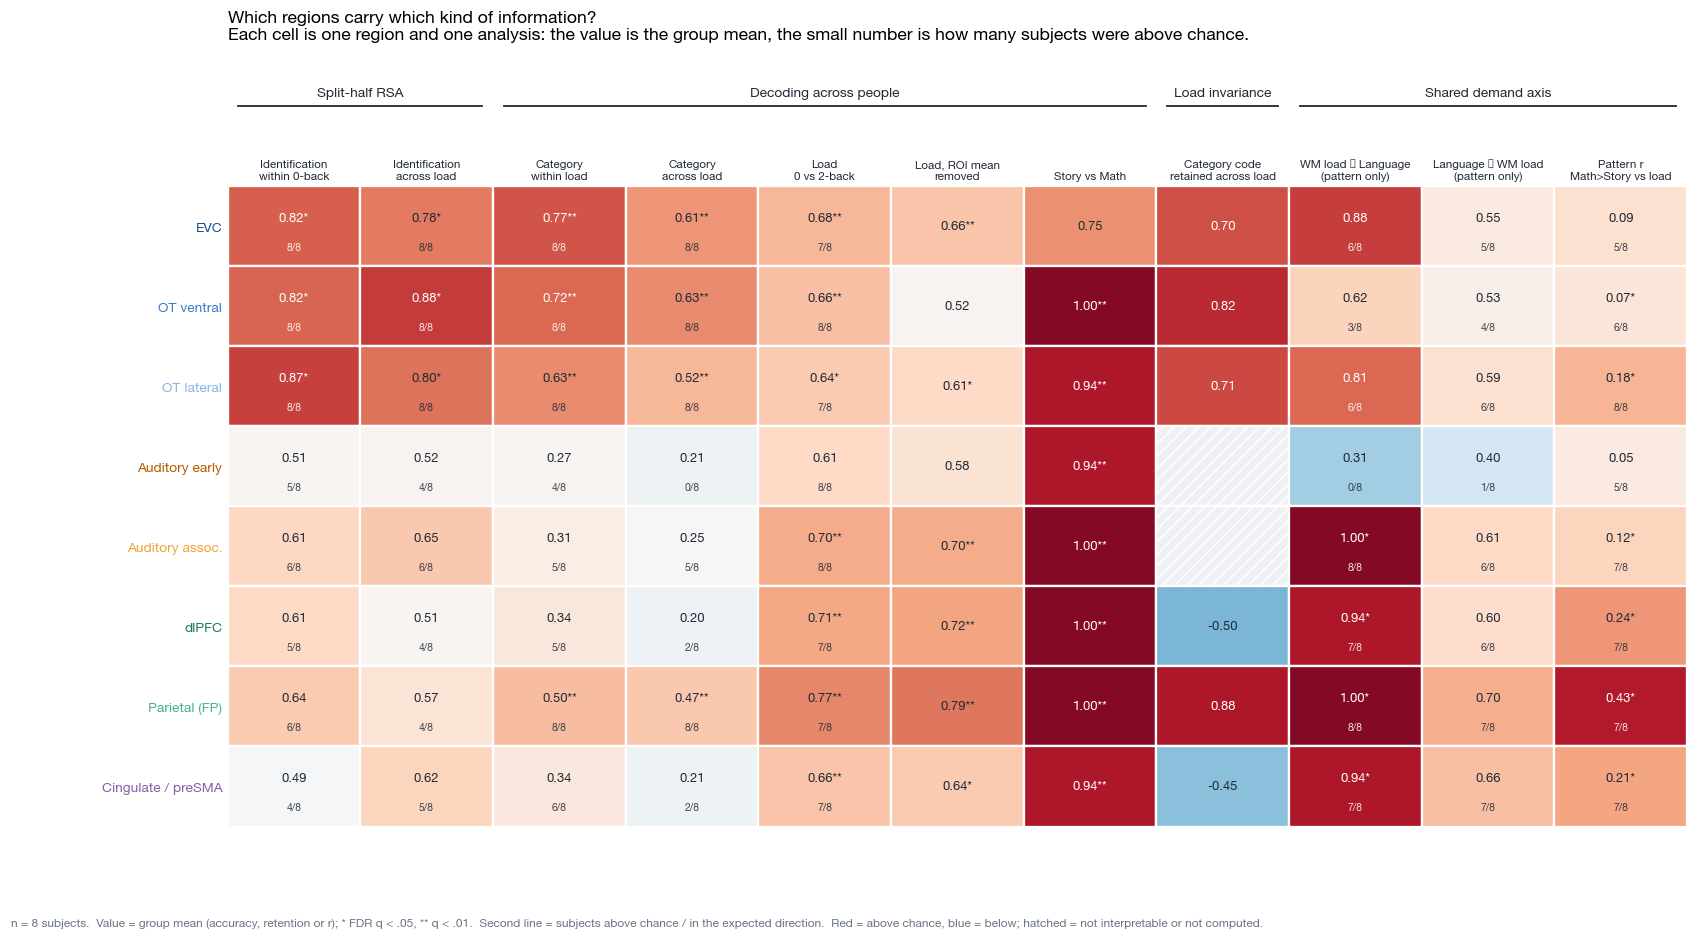
\includegraphics[width=0.85\textwidth]{figures/fig_summary_heatmap.png}
\caption{All main results in one view. Each cell is one region and one analysis: group average, below it the number of people above chance, stars for reliable results; red above chance, blue below, hatched cells could not be interpreted.}
\label{fig:summary}
\end{figure*}

\section{Discussion and Conclusion}
\textbf{What the data show.} Category in early visual and visual-object cortex \cite{haxby2001,kanwisher1997,epstein1998,downing2001} mostly confirms that the analysis works, and the spread signal agrees with \cite{haxby2001}; a similar result in a different dataset is a modest replication. Load was less localised than expected. In prefrontal, parietal and auditory association cortex it is a spatial pattern, fitting a system that serves many demands \cite{duncan2010}; in OT ventral it is an overall activity drop. Parietal category was unexpected, but depends on places blocks tied to timing and did not beat the resting level across loads, so it is a lead, not a finding. The category code survives load largely, but we cannot show fully: accuracy fell by $0.09$--$0.16$ in visual regions and no region passed the ``unchanged'' test, although part of the loss may reflect noisier 2-back data (EVC: $0.72$ against $0.81$). The cross-task results give the clearest support for a shared demand signal: Language timing differs between people, so shared timing is unlikely to explain them, and the pattern correlation points the same way, strongest in parietal cortex; the frontoparietal/sensory split is partial.

\textbf{Novelty and contribution.}\label{sec:novelty} The individual findings agree with earlier work: category patterns in visual cortex \cite{haxby2001}, frontoparietal demand \cite{duncan2010,barch2013} and load-dependent sensory representations \cite{emrich2013}. We do not claim these. We add their combination on one dataset with controls: a model that separates how much of a code is shared across loads from how strong it is, with a test for ``unchanged'' \cite{kriegeskorte2013,bernardi2020,schuirmann1987}; a matched rfMRI control; mean-activity controls in every cross-task decoder \cite{coutanche2013}; a timing audit with schedule-shift and block-position controls; a demand-pattern comparison across two tasks; and a record of two analyses that failed at this sample size.

\textbf{Limitations.} (1) \emph{Small sample:} with eight people the strongest result is that everyone agrees, and showing invariance needs small between-person differences. (2) \emph{Shared WM timing} \cite{haynes2006}: removing places weakens parietal category and shifted timing on resting data did not rescue it. (3) \emph{Incomplete controls:} resting data for four of eight, 100 decoding draws, no spin test, and no places-removed ``unchanged'' test. (4) \emph{ROI sizes} differ about fourfold. (5) \emph{Measurement:} no spatial-noise correction of distances, group parcellation. (6) \emph{No behaviour} data, and hard blocks may differ in effort. (7) \emph{Many tests} were corrected within separate families, so the overall false-positive risk is higher than any single value suggests.

\textbf{Future work.} Add participants (after a power calculation), resting data for everyone with more decoder draws, a places-removed parietal analysis, the spin test, noise-corrected distances, and links to behaviour; a mechanistic model of memory without sustained activity using short-term synaptic plasticity, as in the class models, could then be compared with the data.

\textbf{Conclusion.} In a pilot with eight HCP participants: (1) category can be read out reliably from early visual and visual-object cortex, spread over many locations; (2) load can be read out from most regions, as a spatial pattern in prefrontal, parietal and auditory association cortex and as an overall activity change in OT ventral; (3) the category code is largely kept across load but we could not show it unchanged, and the one region where it looked unchanged, parietal, depends on places blocks and did not beat the resting level, even with shifted timing and block position removed; (4) a load decoder also separates Math from Story in prefrontal, parietal, cingulate and auditory association cortex, most strongly in parietal. The study is limited by sample size, shared timing and resting data for four people; the code runs unchanged on a larger sample.

\section*{Individual Contributions}
The work was shared equally and every part was reviewed and verified by the other author for consistency; both contributed throughout. The primary focus of the 1\textsuperscript{st} author (Sai Veeksha Tavva) was project design and hypotheses, data preparation and the GLM, region definitions and RSA, and cross-subject decoding. The primary focus of the 2\textsuperscript{nd} author (Sahishnu Pawan Kumar) was the load and category-invariance analyses, the resting-state null and schedule controls, the cross-task analyses and figures, and the report and presentation.

\section*{Code Availability}
Code and README: \url{https://github.com/veeksha12/incm-hcp-task-fmri-project}. The notebook \texttt{code-implementation.ipynb} is uploaded already run, so every result and plot can be checked without re-running it (a full run takes a long time). Further plots not shown here are in the supplement, the presentation slides and that notebook.

\begin{thebibliography}{00}
\bibitem{vanessen2013} D. C. Van Essen \emph{et al.}, ``The WU-Minn Human Connectome Project: an overview,'' NeuroImage, vol. 80, pp. 62--79, 2013.
\bibitem{barch2013} D. M. Barch \emph{et al.}, ``Function in the human connectome: task-fMRI and individual differences in behavior,'' NeuroImage, vol. 80, pp. 169--189, 2013.
\bibitem{drobyshevsky2006} A. Drobyshevsky, S. B. Baumann, and W. Schneider, ``A rapid fMRI task battery for mapping of visual, motor, cognitive, and emotional function,'' NeuroImage, vol. 31, pp. 732--744, 2006.
\bibitem{kanwisher1997} N. Kanwisher, J. McDermott, and M. M. Chun, ``The fusiform face area: a module in human extrastriate cortex specialized for face perception,'' J. Neurosci., vol. 17, pp. 4302--4311, 1997.
\bibitem{epstein1998} R. Epstein and N. Kanwisher, ``A cortical representation of the local visual environment,'' Nature, vol. 392, pp. 598--601, 1998.
\bibitem{downing2001} P. E. Downing \emph{et al.}, ``A cortical area selective for visual processing of the human body,'' Science, vol. 293, pp. 2470--2473, 2001.
\bibitem{duncan2010} J. Duncan, ``The multiple-demand (MD) system of the primate brain: mental programs for intelligent behaviour,'' Trends Cogn. Sci., vol. 14, pp. 172--179, 2010.
\bibitem{haxby2001} J. V. Haxby \emph{et al.}, ``Distributed and overlapping representations of faces and objects in ventral temporal cortex,'' Science, vol. 293, pp. 2425--2430, 2001.
\bibitem{kriegeskorte2008} N. Kriegeskorte, M. Mur, and P. Bandettini, ``Representational similarity analysis --- connecting the branches of systems neuroscience,'' Front. Syst. Neurosci., vol. 2, art. 4, 2008.
\bibitem{emrich2013} S. M. Emrich, A. C. Riggall, J. J. LaRocque, and B. R. Postle, ``Distributed patterns of activity in sensory cortex reflect the precision of multiple items maintained in visual short-term memory,'' J. Neurosci., vol. 33, pp. 6516--6523, 2013.
\bibitem{kriegeskorte2013} N. Kriegeskorte and R. A. Kievit, ``Representational geometry: integrating cognition, computation, and the brain,'' Trends Cogn. Sci., vol. 17, pp. 401--412, 2013.
\bibitem{bernardi2020} S. Bernardi \emph{et al.}, ``The geometry of abstraction in the hippocampus and prefrontal cortex,'' Cell, vol. 183, pp. 954--967, 2020.
\bibitem{binder2011} J. R. Binder \emph{et al.}, ``Mapping anterior temporal lobe language areas with fMRI: a multicenter normative study,'' NeuroImage, vol. 54, pp. 1465--1475, 2011.
\bibitem{woolrich2001} M. W. Woolrich, B. D. Ripley, M. Brady, and S. M. Smith, ``Temporal autocorrelation in univariate linear modeling of fMRI data,'' NeuroImage, vol. 14, pp. 1370--1386, 2001.
\bibitem{walther2016} A. Walther \emph{et al.}, ``Reliability of dissimilarity measures for multi-voxel pattern analysis,'' NeuroImage, vol. 137, pp. 188--200, 2016.
\bibitem{nili2014} H. Nili \emph{et al.}, ``A toolbox for representational similarity analysis,'' PLoS Comput. Biol., vol. 10, e1003553, 2014.
\bibitem{coutanche2013} M. N. Coutanche, ``Distinguishing multi-voxel patterns and mean activation: why, how, and what does it tell us?,'' Cogn. Affect. Behav. Neurosci., vol. 13, pp. 667--673, 2013.
\bibitem{haynes2006} J.-D. Haynes and G. Rees, ``Decoding mental states from brain activity in humans,'' Nat. Rev. Neurosci., vol. 7, pp. 523--534, 2006.
\bibitem{stelzer2013} J. Stelzer, Y. Chen, and R. Turner, ``Statistical inference and multiple testing correction in classification-based multi-voxel pattern analysis (MVPA),'' NeuroImage, vol. 65, pp. 69--82, 2013.
\bibitem{nichols2002} T. E. Nichols and A. P. Holmes, ``Nonparametric permutation tests for functional neuroimaging: a primer with examples,'' Hum. Brain Mapp., vol. 15, pp. 1--25, 2002.
\bibitem{glasser2016} M. F. Glasser \emph{et al.}, ``A multi-modal parcellation of human cerebral cortex,'' Nature, vol. 536, pp. 171--178, 2016.
\bibitem{robinson2014} E. C. Robinson \emph{et al.}, ``MSM: a new flexible framework for multimodal surface matching,'' NeuroImage, vol. 100, pp. 414--426, 2014.
\bibitem{salimi2014} G. Salimi-Khorshidi \emph{et al.}, ``Automatic denoising of functional MRI data: combining independent component analysis and hierarchical fusion of classifiers,'' NeuroImage, vol. 90, pp. 449--468, 2014.
\bibitem{benjamini1995} Y. Benjamini and Y. Hochberg, ``Controlling the false discovery rate: a practical and powerful approach to multiple testing,'' J. R. Stat. Soc. B, vol. 57, pp. 289--300, 1995.
\bibitem{schuirmann1987} D. J. Schuirmann, ``A comparison of the two one-sided tests procedure and the power approach for assessing the equivalence of average bioavailability,'' J. Pharmacokinet. Biopharm., vol. 15, pp. 657--680, 1987.
\bibitem{mantel1967} N. Mantel, ``The detection of disease clustering and a generalized regression approach,'' Cancer Res., vol. 27, pp. 209--220, 1967.
\end{thebibliography}

\end{document}
